% cut from impact:






\comment{
- emphasize research domain-independent application (Journal's goals/values page says they prioritize this in submissions)
- applicability not limited to research
    - regression (?) testing
    - ***^^not sure this should be included -- hurts framing of davos as "research software"***
- makes writing and running publicly available reproducible code more accessible (lowers required software comfort/familiarity level \& computing resources vs. installing docker/singularity/conda)
    - also removes these requirements from other scenarios, e.g., easier for new/less experienced students/RAs to get involved with analyses
- mention something about not having to teach environment management to teach day 1 python lesson, or spend hours debugging conda installation in order to share tutorial or demo with students
    - e.g., "researchers who teach \_\_\_ may be familiar with the experience of running a lesson or workshop that requires students to use Docker (or similar...) to run their code, only to spend the majority of class time debugging students' computing environments rather than teaching the lesson itself."
}

Since its initial release, \texttt{davos} has found use in a variety
of applications.  In addition to managing data analysis environments
for multiple ongoing research studies, \texttt{davos} is being used by
both students and instructors in programming courses such as
\href{https://github.com/ContextLab/storytelling-with-data}{\textit{Storytelling
    with Data}} \cite{Mann21b} (an open course on data science,
visualization, and communication) to simplify distributing lessons and
submitting assignments, as well as in online demos such as
{\texttt{abstract2paper}} \cite{Mann21a} (an example application of
\href{https://github.com/EleutherAI/gpt-neo}{GPT-Neo}) to share
ready-to-run code that installs dependencies automatically.

%\textbf{This is the main section of the article and the reviewers weight the description here appropriately}

%Indicate in what way new research questions can be pursued as a result of the software (if any).

%Indicate in what way, and to what extent, the pursuit of existing research questions is improved (if so).

%Indicate in what way the software has changed the daily practice of its users (if so).

%Indicate how widespread the use of the software is within and outside the intended user group.

%Indicate in what way the software is used in commercial settings and/or how it led to the creation of spin-off companies (if so).






% cut from introduction:



% % STOPPED HERE...



% Sharing a project's code base is most valuable when that code may be
% run on 



% Modern scientific research frequently entails writing software code
% for a wide variety of purposes throughout the scientific process.
% Researchers across disciplines may design and implement complex
% experiments; collect, store, and analyze large datasets; create
% visualizations for presentations and publications; and share their
% findings and techniques with peers, students, and the broader public
% through tutorials, demos, workshops, and classes.  However, one
% fundamental requirement of virtually any form of research-related code
% is that its behavior and outputs remain consistent and predictable, no
% matter when, where, or by whom it is run.  This stability can be
% crucial, for example, to ensuring that data are collected under the
% same conditions (e.g., across recordings, subjects, or physical
% locations)
% %^ or locations, e.g., in different test rooms, on different machines, at different sites, etc.
% over multiple months or years, and that they can be accessed,
% processed, and analyzed consistently by a research team that may be
% spread across multiple institutions or countries.  Additionally,
% modern open science practices encourage publicly sharing research code
% and data so that others may explore, reproduce, learn from, and build
% upon existing work.  Much of the benefit afforded by freely available
% research code depends on users' ability to execute it and achieve the
% same result as its original author.

% Python \cite{vanR95} has become one of the most widely used and
% fastest-growing scientific programming languages, in part by combining
% an accessible, high-level syntax with a rich ecosystem of powerful
% third-party tools that facilitate rapid development and collaboration
% \cite{MullEtal15}.  The Python ecosystem offers an extensive data
% science toolkit with platforms for interactive programming (e.g.,
% Project Jupyter \cite{KluyEtal16}, Google Colaboratory),
% community-maintained libraries for data manipulation (e.g., NumPy
% \cite{HarrEtal20}, SciPy \cite{VirtEtal20}, Pandas \cite{McKi10}) and
% visualization (e.g., Matplotlib \cite{Hunt07}, seaborn \cite{Wask21}),
% frameworks for training complex machine learning models (e.g.,
% scikit-learn \cite{PedrEtal11}, TensorFlow \cite{AbadEtal15}, Hugging
% Face~\cite{WolfEtal20}), and myriad other resources.  However, this
% heavy emphasis on third-party libraries also presents a challenge to
% writing and sharing stable, reproducible scientific Python code:
% different versions of the same library may behave differently, adopt
% changes in syntax, expose different functions and interfaces, add or
% drop support for specific hardware or software, write (or expect to
% read) files in different formats, fix (or introduce) bugs, and so on.
% While these issues exist to some extent in any software language or
% ecosystem, they have a particular impact on the Python community due
% to its unusually rapid growth relative to other languages.  Ensuring
% Python code behaves consistently over time and across users therefore
% typically requires ensuring it is always run with the same specific
% set of versions for each third-party package used.
% %Ensuring Python code behaves consistently over time and across users therefore typically requires guaranteeing that the same specific version of each required third-party package is used, every time it is run.

% One common approach to solving this problem is to create containerized
% or virtualized Python environments (e.g., using Docker \cite{Merk14},
% Singularity \cite{KurtEtal17}, or conda \cite{Anac12}) tailored to
% individual applications.  A researcher may build such an environment
% around a particular experiment or analysis pipeline, and exclusively
% run their code from inside it, ``entering" and ``exiting" the
% environment before and after each time they do so.  They can also
% distribute their custom environment alongside their code as a
% configuration file that explicitly lists required package versions,
% enabling others to build identical copies for themselves.  This allows
% research teams to deploy experiments on multiple machines for more
% efficient data collection, collaborate on analyses without introducing
% conflicts or inconsistencies, and publicly share their study designs
% and results for others to reproduce, replicate, or adapt to study new
% questions in the future.

% While often effective, this approach bears two notable drawbacks.
% First, it can add substantially to the technical knowledge, computing
% resources, and initial setup needed to run or share the actual code of
% interest.  For example, sharing code for an analysis or tutorial that
% relies on a particular Docker image to run properly would of course
% necessitate writing and distributing extra configuration files and
% setup instructions.  But far more burdensomely, it also requires that
% anyone who may want to run the code (in addition to the author seeking
% to share it!) first be able to install and navigate additional
% software that is likely far more complex and resource-intensive than
% the actual analysis or tutorial code it facilitates running.  This can
% introduce a need for both a degree of computer literacy and
% computational resources that may not be universally accessible,
% particularly to students or other early-career scientists hoping to
% learn from publicly available tutorials.  These added prerequisites
% clash with the simplicity and accessibility that have contributed to
% Python's popularity, and can create significant barriers to both
% contributing to and taking advantage of open science resources.

% Second, while many existing tools allow users to initially populate a
% Python environment with a fixed set of packages and package versions
% (e.g., from a \texttt{requirements.txt}, \texttt{pyproject.toml},
% \texttt{environment.yml}, \texttt{Pipfile}, \texttt{Dockerfile RUN}
% instruction, etc.), few, if any, ensure that these specified
% requirements \textit{remain} satisfied after they are first installed.
% The ability to modify an environment after its creation is useful in
% many cases (e.g., to install additional software, when
% needed). However, this also makes it easy to inadvertently alter
% existing packages, potentially leading to subtle issues with code that
% relies on them.  For instance, suppose a researcher has implemented a
% series of analyses using version 1.0 of ``Package \textit{X}," and
% decides to perform an additional analysis that requires installing
% ``Package \textit{Y}."  If Package \textit{Y} depends on version 0.9
% of Package \textit{X}, then Package \textit{X} will be downgraded to
% accommodate this new requirement, potentially altering or breaking
% previous analyses when they are rerun later, either by the researcher
% or someone with whom they've shared their code.  Further, if some
% analyses require Package \textit{Y} while others rely on features of
% Package \textit{X} not implemented until version 1.0, it's unclear
% which version the researcher should install in their environment.

% %The \texttt{davos} package provides a novel, Python-native framework for creating, sharing, and running reproducible workflows that was designed to address each of these issues.
% The \texttt{davos} package provides a novel, Python-native framework
% for creating reproducible workflows that was designed to address each
% of these issues. \texttt{davos} allows users to specify dependencies
% directly within the code that...

% \comment {
% POINTS TO MAKE/THINGS TO SAY HERE TO WRAP UP (or maybe save some for impact section?):
% - davos simplifies the process of writing, sharing, and running reproducible code (eliminates need for additional complex env management tools, syntax is simple, packages are just installed at runtime without additional setup beforehand, etc.)...
% - ...it also provides stability/additional protections against accidental changes in ways other tools don't (i.e., addresses issue 2 above) by verifying (and installing if necessary) requirements each time code is run
% - ... while simultaneously enabling new package management patterns (using multiple versions versions of package in same notebook, etc.)
% - it's lightweight and intuitive (unlike big/complex env management tools like docker, etc.)
% - "davos was specifically designed for use with Jupyter notebook environments, and can be used either on its own or in tandem with another environment management tool"
% - "\texttt{davos} was designed specifically for use in Jupyter notebook (formerly called IPython notebook \cite{PereGran07}) environments, and supports Jupyter notebooks \cite{KluyEtal16}, JupyterLab \cite{GranGrou16}, Google Colaboratory, Binder \cite{RagaWill18}, and IDE-based notebook editors."

% - maybe don't mention smuggle statement \& onion comment explicitly in this paragraph since they haven't been defined/explained yet, or if we do, then add some sort of "see \_\_\_ below" with \\ref to relevant subsection
% }


%Introduce the scientific background and the motivation for developing the software.

%Explain why the software is important, and describe the exact (scientific) problem(s) it solves.

%Indicate in what way the software has contributed (or how it will contribute in the future) to the process of scientific discovery; if available, this is to be supported by citing a research paper using the software.

%Provide a description of the experimental setting (how does the user use the software?).

%Introduce related work in literature (cite or list algorithms used, other software etc.).





% ABSTRACT:

%Many important parts of modern scientific research depend on writing, sharing, and running reproducible code. It enables scientists to collaborate on projects, replicate and extend prior work, and teach students new ideas and techniques through hands-on, interactive tutorials.

%The ability to write, share, and run reproducible code plays many important roles in modern scientific research:

%Writing and sharing reproducible code plays an important role in modern scientific research, enabling scientists to collaborate on projects, replicate and extend previous work, and teach students concepts and techniques through

%\texttt{davos} is a Python package that provides a simple, accessible, and effective way to manage and share reproducible code.

%\texttt{davos} provides the \texttt{smuggle} statement

%\texttt{davos} is a Python package that allows users to write, run, and share reproducible Python code without the need for containers or virtual environments.

%davos is a Python package that allows users to manage and share reproducible code without the need for containers or virtual environments.

%\texttt{davos} is a Python package for creating, running, and sharing reproducible workflows without the need for external containerized or virtualized environments.

%\texttt{davos} is a Python package that makes writing, running, and sharing reproducible code easy. Importing \texttt{davos} in an IPython notebook enables the \textit{smuggle} statement: a drop-in replacement for the built-in \textit{import} statement that can install missing packages as needed at runtime, and may be

%\texttt{davos} is a Python package for creating self-managing, reproducible workflows that specify dependencies directly within their code and install packages as needed at runtime.

%\texttt{davos} works by providing the \textit{smuggle} statement: a drop-in replacement for the built-in \texttt{import} statement that  \_\_\_, and the

% \texttt{davos} is a Python package for creating self-managing, reproducible workflows that specify dependencies directly in their code, and install them
% \texttt{davos} is a Python package that enables creating and sharing reproducible workflows as a single, ready-to-run IPython notebook.

%davos is a python package for creating, sharing, and running reproducible code without the need for


% ========================================================================================================


% Modern open science practices promote sharing code and data to enable others to explore, reproduce, learn from, and build upon existing work. Scientists, researchers, and educators produce many different forms of research-related code (e.g., experiments, data analyses, tutorials, demos) that they may seek to share with a wide range of audiences including collaborators, students, the broader scientific community, and the general public. Python has become one of the most widely used and fastest-growing scientific programming languages as it offers both a simple, accessible grammar and an extensive 

%Modern scientific research frequently involves writing code for different purposes throughout the research process (e.g., experiments, data analyses, tutorials, or demos). A nearly universal (but often challenging) requirement of research-related code is that its behavior and outputs must remain consistent every time it is run, both over time and across users. This stability can be crucial to ensuring that data are collected under identical conditions (e.g., across recordings, trials, or subjects) and that statistical analyses yield accurate, consistent results. Additionally, modern open science practices encourage sharing code and data publicly to enable others to explore, reproduce, learn from, and build upon existing work. Scientists, researchers, and educators may seek to share research-related code with a wide range of audiences including collaborators, students, the broader scientific community, and the general public.

%Modern scientific research often involves writing code that must behave consistently every time it is run. For example, stable code can be crucial to ensuring data are collected under the same conditions, recorded and processed in a common format, and yield reliable results when analyzed. Additionally, modern open science practices promote sharing code and data to enable others to explore, reproduce, learn from, and build upon existing work. Scientists, researchers, and educators produce many different forms of research-related code (e.g., experiments, data analyses, tutorials, demos) that they may seek to share with a wide range of audiences including collaborators, students, the broader scientific community, and the general public. 

%%Modern scientific research frequently involves writing code for different purposes throughout the research process (e.g., experiments, data analyses, tutorials, or demos). An often essential (but often challenging) part of writing code for scientific research is ensuring its behavior and outputs remain consistent every time it is run, both over time and across users.

% Modern scientific research often involves writing code for various uses throughout the research process (e.g., experiments, data analyses, tutorials, and demos). An often-essential feature of research-related code is that it must behave consistently 

% A common challenge when writing 

%A common requirement of code written for scientific research is that it must behave consistently every time it is run. This 

% Modern scientific research frequently involves writing code whose behavior and outputs must be consistent every time it is run. This stability is essential for 

%When writing code for scientific research, it is often essential to ensure that the code 

%Modern scientific research frequently involves writing code whose behavior must be consistent every time it is run. This stability is essential to ensuring 

%An essential part of modern scientific research is writing code that behaves consistently every time it is run. Stable code is crucial to ensuring data are collected under the same conditions across trials, subjects, or observations; recorded and processed in a standard format; 

%For example, stable code helps ensure data are collected, recorded, and processed consistently, and that analyses performed on those data yield reliable results. 

%Code that remains stable over time is essential to ensuring that data are collected under constant conditions, recorded and stored in a standard format, and yield accurate results when analyzed.

%For example, stable code helps ensure all data are collected under consistent conditions, recorded and stored in a consistent format, and treated consistently during analyses.
 
% An essential feature of software used in scientific research is that it behaves consistently every time it is run. For example, stable code can be crucial to ensuring constant conditions during data collection (e.g., across recordings, trials, or subjects) and that accurate, reliable outputs from statistical analyses. Additionally, modern open science practices encourage sharing code and data to enable others to explore, reproduce, learn from, and build upon existing work. Scientists, researchers, and educators produce many different forms of research-related code (e.g., experiments, analyses, tutorials, and demos) that they may seek to share with a wide range of audiences including collaborators, students, the broader scientific community, and the general public.

%Modern scientific research often involves writing code for various purposes throughout the research process, from designing experiments to performing data analyses to presenting results through tutorials or demos. A nearly universal requirement of any form of research-related code is that its behavior and outputs must remain consistent every time it is run, both over time and across users. This stability can be crucial to ensuring that data are collected under identical conditions (e.g., across recordings, trials, or subjects) and that statistical analyses yield accurate, consistent results. Additionally, open science practices encourage sharing code and data publicly to enable others to explore, reproduce, learn from, and build upon existing work. Scientists, researchers, and educators may seek to share research-related code with a wide range of audiences including collaborators, students, the broader scientific community, and the general public.

%Modern scientific research often involves writing code throughout the research process, from designing experiments, to analyzing data, to presenting findings via tutorials or public demos. 

%Modern scientific research frequently entails writing software code for a wide range of purposes throughout the research process, from designing experiments, to processing and analyzing data, to sharing results and techniques with peers or students through tutorials, demos, workshops, and classes. One requirement common to nearly all research-related code it that its behavior and/or outputs remain consistent and predictable every time it is run, both over time and across different users. For instance, this stability can be crucial to ensuring that data are collected under the same conditions (e.g., across recordings, trials, or subjects) and that statistical analyses yield accurate, reliable results. 

%However, one requirement common to virtually all forms of research-related code is that it behave consistently and predictably every time it is run, both over time and across users.
%This stability can be crucial, for example, to carrying out studies that span multiple years or institutions
%This stability can be crucial to ensuring, for example, that data are collected under the same conditions (e.g., across recordings, trials, or subjects) over multiple months or years, and can be accessed, processed, and analyzed consistently by collaborators across multiple institutions or countries.

%For example, this stability can be crucial to ensuring that data are collected under the same conditions (e.g., across recordings, trials, or subjects), preprocessed in the same manner, stored in a standardized format, and treated equitably by statistical analyses.
%This stability can be crucial to ensuring, for example, that data are collected under constant conditions (e.g., across recordings, trials, or subjects), are preprocessed and stored in a standard format, and that they can be easily accessed and consistently analyzed by collaborators across multiple institutions or countries.

%Scientists, researchers, and educators may seek to share research code with audiences that have a broad range of scientific and technical backgrounds, including collaborators, students, 
%stakeholders, 
%the broader scientific community, and the general public.


% ========================================================================================================


%Python has become one of the most widely used and fastest-growing scientific programming languages \cite{MullEtal15}, in part due to its accessible, high-level grammar and extensive ecosystem of powerful third-party data science tools, including platforms for interactive development (e.g., Project Jupyter, \cite{KluyEtal16}; Google Colaboratory), community-maintained libraries for data manipulation (e.g., \texttt{NumPy} \cite{HarrEtal20}, \texttt{SciPy} \cite{VirtEtal20}, \texttt{Pandas} \cite{McKi10}) and visualization (e.g., \texttt{Matplotlib} \cite{Hunt07}, \texttt{seaborn} \cite{Wask21}), and myriad other software. However, this heavy use of third-party packages also presents a challenge to writing and sharing stable, reproducible scientific Python code: different versions of the same third-party library can behave differently, use different syntax, add or drop support for specific functions or other libraries, address (or introduce) bugs, and so on. While these issues are present to some extent in any language or ecosystem, they have a particular impact on the Python community due to its unusually rapid growth relative to other languages. Ensuring consistent behavior over time and across users therefore typically requires ensuring that code is shared and run with a specific set of versions for each package used. 

%the availability of powerful third-party tools \cite{MullEtal15} . 
%an extensive ecosystem of third-party tools \cite{MullEtal15}.

%Python \cite{vanR95} has become one of the most widely used and fastest-growing scientific programming languages by combining an accessible, high-level syntax with the availability of powerful third-party tools that facilitate rapid development and collaboration \cite{MullEtal15}.


%However, this heavy emphasis on third-party libraries also presents a challenge to writing and sharing stable, reproducible scientific Python code: different versions of the same library may behave differently, adopt changes in syntax, add or drop support for specific functions or other libraries, save data in (and expect loaded data to adhere to) different formats, address (or introduce) bugs, and so on.

%Ensuring Python code behaves consistently over time and across users therefore typically requires making sure it is always run with the same specific set of versions for each package used.


% ========================================================================================================


%They can also distribute this custom environment alongside their code as a configuration file that explicitly lists required package versions, enabling others to build identical copies for themselves.

% ========================================================================================================

%For example, sharing an analysis or tutorial that relies on a particular Docker image to run properly not only necessitates writing and distributing extra configuration files and setup instructions, but more significantly, requires anyone hoping to run code (including the original author) to first be able to install and navigate additional software that is likely far more complex and resource-intensive than the actual analysis or tutorial code it facilitates running.

%For example, sharing an analysis or tutorial that relies on a particular Docker image to run properly not only necessitates distributing extra configuration files and setup instructions, but also requires both the original author and anyone with whom the code is shared to first install and navigate additional software that is likely more complex and resource-intensive than the actual code it facilitates running.

%For example, sharing an analysis or tutorial that relies on a particular Docker image to run properly necessarily requires writing and distributing extra configuration files and setup instructions. But more significantly, it also requires that anyone seeking to run the code first be able to install and navigate additional software that is likely far more complex and resource-intensive than the actual analysis or tutorial it facilitates running.

%For example, sharing an analysis or tutorial that relies on a particular Docker image to run properly would, of course, necessitate writing and distributing extra configuration files (e.g., a \texttt{Dockerfile} or \texttt{docker-compose.yaml}) as well as initial setup instructions. %While this may be a mere minor inconvenience (if not a fact of everyday life) for users seasoned in DevOps tooling, the impact is far more significant in a research context, requiring both the original author and anyone else who may want to run their code (whether Z

% ========================================================================================================


% First, most tools for building a Python environment from a configuration file (e.g., ..) work by installing all requirements upfront, but typically do not enforce their presence after this initial setup. This makes it easy to inadvertently alter the environment after this initial setup. For example, suppose a researcher has implemented a series of analyses using version 1.0 of ``Package \textit{X}," and decides to perform an additional analysis that requires ``Package \textit{Y}." If Package \textit{Y} depends on version 1.1 of Package \textit{X}, then Package \textit{X} will be upgraded to accommodate this new requirement, potentially leading to inconsistent behavior of code that uses Package \textit{X}.

%Second, it can add substantially to the technical knowledge, system resources, and initial setup required to share and run the actual code of interest. For example, sharing research code that relies on a particular Docker image to run properly not only necessitates additional configuration files and setup steps, but also requires both the author and all users with whom it may be shared to install and navigate additional software that is likely more complicated and resource-intensive than the actual code being shared.

% While effective, such tools can add a significant degree of complexity to the process of sharing research code for both the author and 


% ========================================================================================================


%Second, typical environment management tools don't enforce that specified requirements \textit{remain} satisfied after they are initially installed. 

%This makes it easy to inadvertently alter existing packages in a Python environment at any point in time, potentially affecting the behavior of code that depends on them. 

%For instance, suppose a researcher has implemented a series of analyses using version 1.0 of ``Package \textit{X}," and decides to  perform an additional analysis that requires installing ``Package \textit{Y}." 

%If Package \textit{Y} depends on version 1.1 of Package \textit{X}, then Package \textit{X} will be upgrade to accommodate this new requirement, potentially altering or breaking the previous analyses in future runs, as well as for anyone with whom  analysis code. 

%Further, if earlier analyses require functionality 

%install a fixed set of required Python packages in an isolated environment (e.g., from a \texttt{requirements.txt}, \texttt{pyproject.toml}, \texttt{environment.yml}, \texttt{Pipfile}, \texttt{Dockerfile RUN} instruction, etc.), few, if any, enforce that the specified requirements \textit{remain} satisfied after this initial setup.


% ========================================================================================================


%\texttt{davos} was created\comment{designed?} to address these issues by providing a novel, Python-native framework for creating, sharing, and running reproducible workflows. The general scheme for using \textit{davos} (described in \hyperref[sec:functionalities]{\textit{Software functionalities}}, below) was designed with \textbf{NUMBER} goals in mind: to be more accessible, intuitive, and lightweight than typical environment management tools; to guarantee the desired version

%We created the davos package \comment{the davos package was created} to address these issues by providing a novel, Python-based \comment{Python-native(?)} framework for writing, sharing, and running reproducible code. davos was designed with the goal of stimultaneously being being more accessible, intuitive, and lightweight than typical environment management tools; guaranteeing that Python workflows always use the intended package versions (even beyond their initial installation); providing greater, more precise control over which package versions are used for what purposes

%We created \texttt{davos} to address these issues, with the goal of providing an alternative approach to ensuring reproducibility over time and across users that is more intuitive

%The \texttt{davos} package was designed to address these issues by providing an intuitive, lightweight, and Python-native way to ensure reproducibility over time and across users. With \texttt{davos} users to distribute reproducible workflows as a single, ready-to-run Jupyter notebook \cite{KluyEtal16} that specifies


% ========================================================================================================


%For greater control over the behavior of \texttt{smuggle} statements, \texttt{davos} defines an additional construct called the ``onion comment''. An onion comment is a special type of inline comment that may be placed on a line containing a \texttt{smuggle} statement to customize how \texttt{davos} searches for the smuggled package locally and, if necessary, downloads and installs it. Onion comments follow a simple syntax based on the ``type comment'' syntax introduced in PEP 484 \cite{vanREtal14}, and are designed to make managing packages with \texttt{davos} intuitive and familiar. To construct an onion comment, simply provide the name of the installer program (e.g., \texttt{pip}) and the same arguments one would use to manually install the package as desired via the command line\comment{(see Fig.~\ref{fig:snippets})} (see Fig.~\ref{fig:snippets}, lines 3--10 for examples).

%Onion comments are useful when smuggling a package whose distribution name (i.e., the name used when installing it) is different from its top-level module name (i.e., the name used when importing it; e.g., Fig.~\ref{fig:snippets}, lines 12--13). However, the most powerful use of the onion comment is making \texttt{smuggle} statements \textit{version-sensitive}. If an onion comment includes a version specifier \cite{CoghStuf13} (e.g., Fig.~\ref{fig:snippets}, lines 15--19), \texttt{davos} will ensure that the version of the package loaded into the notebook always matches the specific version requested, or satisfies the given version constraints. If the smuggled package exists locally, \texttt{davos} will extract its version info from its metadata and compare it to the specifier provided. If the two are incompatible (or no local installation is found), \texttt{davos} will install and load a suitable version of the package instead. Onion comments can similarly be used to smuggle specific VCS references (e.g., Git \cite{TorvHama05}  branches, commits, tags, etc.; Fig.~\ref{fig:snippets}, lines 21--22).

%\texttt{davos} processes onion comments internally before forwarding arguments to the installer program. In addition to preventing onion comments from being used as a vehicle for shell injection attacks, this allows \texttt{davos} take certain logical actions when particular arguments are passed (e.g., Fig.~\ref{fig:snippets}, lines 24--28). For example, the \texttt{--force-reinstall}, \texttt{-I}/\texttt{--ignore-installed}, and \texttt{-U}/\texttt{--upgrade} flags will all cause \texttt{davos} to skip searching for a smuggled package locally before installing a new copy; \texttt{--no-input} will temporarily enable \texttt{davos}'s non-interactive mode (see Section \ref{subsec:onion}); and installing a package into \texttt{<dir>} with \texttt{--target <dir>} will cause \texttt{dir} to be prepended to the module search path (\texttt{sys.path}), if necessary, so the package can be imported.

%\begin{figure}[h]
%\centering
%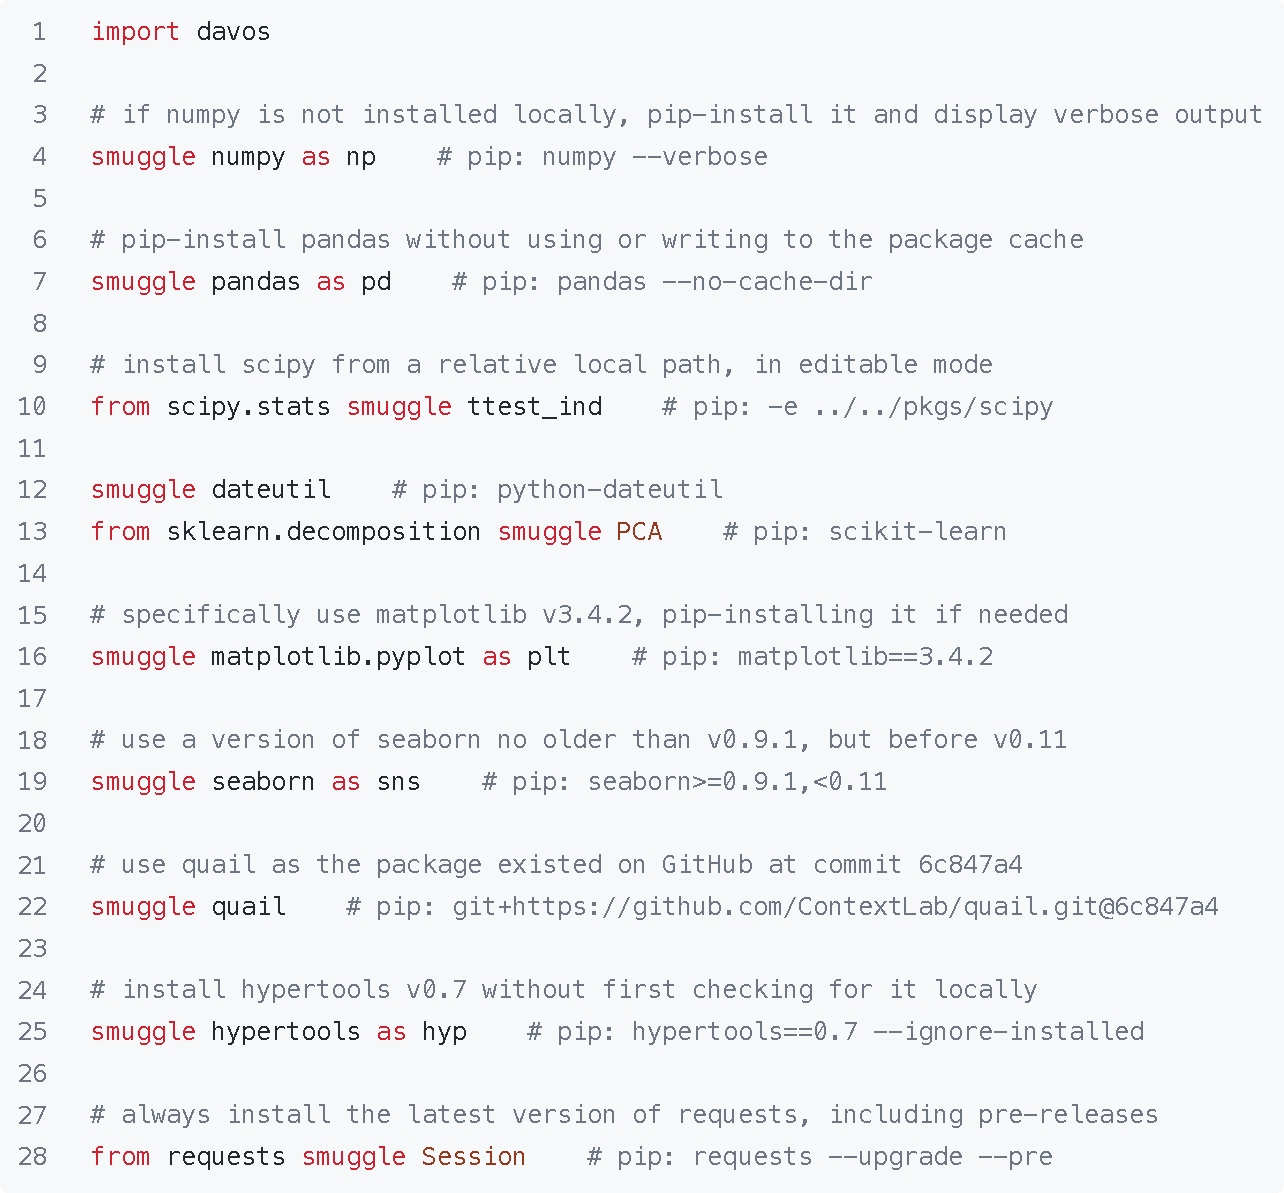
\includegraphics[width=\textwidth]{figs/snippets.pdf}
%\caption{\small Example \texttt{smuggle} statements and accompanying onion comments.}
%\label{fig:snippets}
%\end{figure}




%If an onion comment includes a version specifier (\cite{CoghStuf13}; e.g., Fig.~\ref{fig:snippets}, lines \_\_\_-\_\_\_), \texttt{davos} will first check whether the smuggled package exists locally, and if so, extract its version info from its metadata to compare against the requested version. If the installed version doesn't satisfy the given constraint (or if no local version is found), \texttt{davos} will install and load a suitable version instead. This guarantees the notebook is always run with a specific (or constrained) version of a particular package. Similarly, \texttt{davos}
%If the package exists locally, \texttt{davos} will extract its version from metadata before loading it to determine its version, and if it does not match the requested version (or if no local installation is found),
%If an onion comment includes a version specifier \cite{CoghStuf13}, \texttt{davos} will check whether the smuggled package is installed locally (as usual), and if so, additionally parse its metadata to determine
%Adding a version specifier \cite{CoghStuf13} to an onion comment guarantees the version loaded into the notebook will matches the version specified



% ========================================================================================================


%Functionally, importing \texttt{davos} appears to add "\texttt{smuggle}'' to Python's set of reserved keywords (like \texttt{import}, \texttt{def}, \texttt{return}, etc.) and cause comments to be parsed at runtime, when they're otherwise not. However, \texttt{davos} doesn't actually modify 

%Functionally, importing \texttt{davos} appears to create a new reserved Python keyword (like \texttt{import}, \texttt{def}, or \texttt{return}) and cause comments affect runtime behavior, which they normally do not. However, \texttt{davos} doesn't actually modify the rules of Python's parser and lexical analyzer in order to do so---in fact, modifying the Python grammar isn't possible at runtime and would require rebuilding the interpreter. Instead, \texttt{davos} 
% Functionally, importing \texttt{davos} appears to make "\texttt{smuggle}'' a valid Python keyword (like ``\texttt{import}'', ``\texttt{def}'', or ``\texttt{return}'') as well as cause Python to  
% Functionally, importing \texttt{davos} appears to create a new reserved Python keyword, ``\texttt{smuggle}'', similar to ``\texttt{import}'', ``\texttt{def}'', or ``\texttt{return}''.
% Functionally, importing \texttt{davos} appears to add ``\texttt{smuggle}'' to Python's reserved keywords (like ``\texttt{import}'', ``\texttt{def}'', and ``\texttt{return}''). It also appears to cause comments to be parsed, their contents to be potentially relevant to the code's behavior at runtime, which they normally are not.
%It also appears to cause comments to be parsed and capable of affecting code behavior at runtime, which they normally are not. 
%It also appears to cause Python to fundamentally redefine comments as potentially relevant to code behavior at runtime, which they normally are not. 


% ========================================================================================================


%\definecolor{backgroundgrey}{RGB}{244,246,249}
%\definecolor{commentgrey}{RGB}{91,99,110}
%\definecolor{keywordred}{RGB}{194,11,36}
%
%\lstset{
%    backgroundcolor=\color{backgroundgrey},
%    basicstyle=\footnotesize\fontfamily{qag}\selectfont, %\ttfamily,
%    breaklines=true,
%    commentstyle=\color{commentgrey},
%    language=Python,
%    emph={import, smuggle, from, as},
%    emphstyle=\color{keywordred},
%}
%
%\begin{lstlisting}
%import davos
%
%# if numpy is not installed locally, pip-install it and display verbose output
%smuggle numpy as np    # pip: numpy --verbose
%
%# pip-install pandas without using or writing to the package cache
%smuggle pandas as pd    # pip: pandas --no-cache-dir
%
%# install scipy from a relative local path, in editable mode
%from scipy.stats smuggle ttest_ind # pip: -e ../../pkgs/scipy
%\end{lstlisting}

